%======================================================================
% University of Waterloo Thesis Template for LaTeX 
% Last Updated November, 2020 
% by Stephen Carr, IST Client Services, 
% University of Waterloo, 200 University Ave. W., Waterloo, Ontario, Canada
% FOR ASSISTANCE, please send mail to request@uwaterloo.ca

% DISCLAIMER
% To the best of our knowledge, this template satisfies the current uWaterloo thesis requirements.
% However, it is your responsibility to assure that you have met all requirements of the University and your particular department.

% Many thanks for the feedback from many graduates who assisted the development of this template.
% Also note that there are explanatory comments and tips throughout this template.
%======================================================================
% Some important notes on using this template and making it your own...

% The University of Waterloo has required electronic thesis submission since October 2006. 
% See the uWaterloo thesis regulations at
% https://uwaterloo.ca/graduate-studies/thesis.
% This thesis template is geared towards generating a PDF version optimized for viewing on an electronic display, including hyperlinks within the PDF.

% DON'T FORGET TO ADD YOUR OWN NAME AND TITLE in the "hyperref" package configuration below. 
% THIS INFORMATION GETS EMBEDDED IN THE PDF FINAL PDF DOCUMENT.
% You can view the information if you view properties of the PDF document.

% Many faculties/departments also require one or more printed copies. 
% This template attempts to satisfy both types of output. 
% See additional notes below.
% It is based on the standard "book" document class which provides all necessary sectioning structures and allows multi-part theses.

% If you are using this template in Overleaf (cloud-based collaboration service), then it is automatically processed and previewed for you as you edit.

% For people who prefer to install their own LaTeX distributions on their own computers, and process the source files manually, the following notes provide the sequence of tasks:
 
% E.g. to process a thesis called "mythesis.tex" based on this template, run:

% pdflatex mythesis	-- first pass of the pdflatex processor
% bibtex mythesis	-- generates bibliography from .bib data file(s)
% makeindex         -- should be run only if an index is used 
% pdflatex mythesis	-- fixes numbering in cross-references, bibliographic references, glossaries, index, etc.
% pdflatex mythesis	-- it takes a couple of passes to completely process all cross-references

% If you use the recommended LaTeX editor, Texmaker, you would open the mythesis.tex file, then click the PDFLaTeX button. Then run BibTeX (under the Tools menu).
% Then click the PDFLaTeX button two more times. 
% If you have an index as well,you'll need to run MakeIndex from the Tools menu as well, before running pdflatex
% the last two times.

% N.B. The "pdftex" program allows graphics in the following formats to be included with the "\includegraphics" command: PNG, PDF, JPEG, TIFF
% Tip: Generate your figures and photos in the size you want them to appear in your thesis, rather than scaling them with \includegraphics options.
% Tip: Any drawings you do should be in scalable vector graphic formats: SVG, PNG, WMF, EPS and then converted to PNG or PDF, so they are scalable in the final PDF as well.
% Tip: Photographs should be cropped and compressed so as not to be too large.

% To create a PDF output that is optimized for double-sided printing: 
% 1) comment-out the \documentclass statement in the preamble below, and un-comment the second \documentclass line.
% 2) change the value assigned below to the boolean variable "PrintVersion" from " false" to "true".

%======================================================================
%   D O C U M E N T   P R E A M B L E
% Specify the document class, default style attributes, and page dimensions, etc.
% For hyperlinked PDF, suitable for viewing on a computer, use this:
\documentclass[letterpaper,12pt,titlepage,oneside,final]{book}
 
% For PDF, suitable for double-sided printing, change the PrintVersion variable below to "true" and use this \documentclass line instead of the one above:
%\documentclass[letterpaper,12pt,titlepage,openright,twoside,final]{book}

% Some LaTeX commands I define for my own nomenclature.
% If you have to, it's easier to make changes to nomenclature once here than in a million places throughout your thesis!
\newcommand{\package}[1]{\textbf{#1}} % package names in bold text
\newcommand{\cmmd}[1]{\textbackslash\texttt{#1}} % command name in tt font 
\newcommand{\href}[1]{#1} % does nothing, but defines the command so the print-optimized version will ignore \href tags (redefined by hyperref pkg).
%\newcommand{\texorpdfstring}[2]{#1} % does nothing, but defines the command
% Anything defined here may be redefined by packages added below...

% This package allows if-then-else control structures.
\usepackage{ifthen}
\newboolean{PrintVersion}
\setboolean{PrintVersion}{false}
% CHANGE THIS VALUE TO "true" as necessary, to improve printed results for hard copies by overriding some options of the hyperref package, called below.

%\usepackage{nomencl} % For a nomenclature (optional; available from ctan.org)
\usepackage{amsmath,amssymb,amstext} % Lots of math symbols and environments
\usepackage[pdftex]{graphicx} % For including graphics N.B. pdftex graphics driver 

% Hyperlinks make it very easy to navigate an electronic document.
% In addition, this is where you should specify the thesis title and author as they appear in the properties of the PDF document.
% Use the "hyperref" package 
% N.B. HYPERREF MUST BE THE LAST PACKAGE LOADED; ADD ADDITIONAL PKGS ABOVE
\usepackage[pdftex,pagebackref=false]{hyperref} % with basic options
%\usepackage[pdftex,pagebackref=true]{hyperref}
		% N.B. pagebackref=true provides links back from the References to the body text. This can cause trouble for printing.
\hypersetup{
    plainpages=false,       % needed if Roman numbers in frontpages
    unicode=false,          % non-Latin characters in Acrobat’s bookmarks
    pdftoolbar=true,        % show Acrobat’s toolbar?
    pdfmenubar=true,        % show Acrobat’s menu?
    pdffitwindow=false,     % window fit to page when opened
    pdfstartview={FitH},    % fits the width of the page to the window
    pdftitle={Using cosmic-ray hodoscope data to validate the misalignment model of small-strip thin gap chambers for the ATLAS new small wheels},
    pdfauthor={Lia Formenti},
    pdfsubject={Using cosmic-ray hodoscope data to validate the misalignment model of small-strip thin gap chambers for the ATLAS new small wheels},
%    pdfkeywords={keyword1} {key2} {key3}, % list of keywords, and uncomment this line if desired
    pdfnewwindow=true,      % links in new window
    colorlinks=true,        % false: boxed links; true: colored links
    linkcolor=blue,         % color of internal links
    citecolor=green,        % color of links to bibliography
    filecolor=magenta,      % color of file links
    urlcolor=cyan           % color of external links
}
\ifthenelse{\boolean{PrintVersion}}{   % for improved print quality, change some hyperref options
\hypersetup{	% override some previously defined hyperref options
%    colorlinks,%
    citecolor=black,%
    filecolor=black,%
    linkcolor=black,%
    urlcolor=black}
}{} % end of ifthenelse (no else)

\usepackage[automake,toc,abbreviations]{}
% \usepackage[automake,toc,abbreviations]{glossaries-extra} % Exception to the rule of hyperref being the last add-on package
% If glossaries-extra is not in your LaTeX distribution, get it from CTAN (http://ctan.org/pkg/glossaries-extra), 
% although it's supposed to be in both the TeX Live and MikTeX distributions. There are also documentation and 
% installation instructions there.

% Setting up the page margins...
% uWaterloo thesis requirements specify a minimum of 1 inch (72pt) margin at the
% top, bottom, and outside page edges and a 1.125 in. (81pt) gutter margin (on binding side). 
% While this is not an issue for electronic viewing, a PDF may be printed, and so we have the same page layout for both printed and electronic versions, we leave the gutter margin in.
% Set margins to minimum permitted by uWaterloo thesis regulations:
\setlength{\marginparwidth}{0pt} % width of margin notes
% N.B. If margin notes are used, you must adjust \textwidth, \marginparwidth
% and \marginparsep so that the space left between the margin notes and page
% edge is less than 15 mm (0.6 in.)
% \setlength{\marginparsep}{0.125pt} % width of space between body text and margin notes
% Changed even/oddsidemargin from 0.125 to 0 because I think I will only make an electronic copy. Changed textwidth to match. - LF
\setlength{\evensidemargin}{0in} % Adds 1/8 in. to binding side of all 
% even-numbered pages when the "twoside" printing option is selected
\setlength{\oddsidemargin}{0in} % Adds 1/8 in. to the left of all pages when "oneside" printing is selected, and to the left of all odd-numbered pages when "twoside" printing is selected
\setlength{\textwidth}{6.5in} % assuming US letter paper (8.5 in. x 11 in.) and side margins as above
\raggedbottom

% The following statement specifies the amount of space between paragraphs. Other reasonable specifications are \bigskipamount and \smallskipamount.
\setlength{\parskip}{\medskipamount}

% The following statement controls the line spacing.  
% The default spacing corresponds to good typographic conventions and only slight changes (e.g., perhaps "1.2"), if any, should be made.
\renewcommand{\baselinestretch}{1} % this is the default line space setting

% Commented out because you aren't printing and this is a waste of paper - LF
% By default, each chapter will start on a recto (right-hand side) page.
% We also force each section of the front pages to start on a recto page by inserting \cleardoublepage commands.
% In many cases, this will require that the verso (left-hand) page be blank, and while it should be counted, a page number should not be printed.
% The following statements ensure a page number is not printed on an otherwise blank verso page.
% \let\origdoublepage\cleardoublepage
% \newcommand{\clearemptydoublepage}{%
%  \clearpage{\pagestyle{empty}\origdoublepage}}
% \let\cleardoublepage\clearemptydoublepage

% Define Glossary terms (This is properly done here, in the preamble and could also be \input{} from a separate file...)
% \input{glossaries}
% \makeglossaries

%======================================================================
%   L O G I C A L    D O C U M E N T
% The logical document contains the main content of your thesis.
% Being a large document, it is a good idea to divide your thesis into several files, each one containing one chapter or other significant chunk of content, so you can easily shuffle things around later if desired.
%======================================================================
\begin{document}

%----------------------------------------------------------------------
% FRONT MATERIAL
% title page,declaration, borrowers' page, abstract, acknowledgements,
% dedication, table of contents, list of tables, list of figures, nomenclature, etc.
%----------------------------------------------------------------------
% T I T L E   P A G E
% -------------------
% Last updated October 23, 2020, by Stephen Carr, IST-Client Services
% The title page is counted as page `i' but we need to suppress the
% page number. Also, we don't want any headers or footers.
\pagestyle{empty}
\pagenumbering{roman}

% The contents of the title page are specified in the "titlepage"
% environment.
\begin{titlepage}
        \begin{center}
        \vspace*{1.0cm}

        \Huge
        {\bf Cosmic ray validation of electrode positions in small-strip thin gap chambers for the upgrade of the ATLAS detector } \\

        \vspace*{1.0cm}

        \Large
        Lia Formenti \\
        
        \vspace*{1.0cm}
        
        \normalsize
        Department of Physics \\
        McGill University, Montreal \\
        October, 2021 \\

        \vspace*{3.0cm}

        \normalsize
        A thesis submitted to\\
        McGill University \\ 
        in partial fulfillment of the \\
        requirements of the degree of \\
        Master of Science \\

        \vspace*{2.0cm}

        \copyright\ Lia Formenti 2021 \\
        \end{center}
\end{titlepage}

% The rest of the front pages should contain no headers and be numbered using Roman numerals starting with `ii'
\pagestyle{plain}
\setcounter{page}{2}

\cleardoublepage % Ends the current page and causes all figures and tables that have so far appeared in the input to be printed.
% In a two-sided printing style, it also makes the next page a right-hand (odd-numbered) page, producing a blank page if necessary.

% T A B L E   O F   C O N T E N T S
% ---------------------------------
\renewcommand\contentsname{Table of Contents}
\tableofcontents
\cleardoublepage
\phantomsection    % allows hyperref to link to the correct page

% A B S T R A C T
% ---------------

\begin{center}\textbf{Abstract}\end{center}
% Medium length abstract
% The particle collision rate at the Large Hadron Collider (LHC) will be effectively increased in 2025-2027 by an extensive upgrade program. The upgrades will improve the statistics on measurements and the sensitivity of searches for rare processes using the ATLAS experiment and other experiments at the LHC. The innermost endcaps of the ATLAS muon spectrometer consist of two wheels of muon detectors that must be replaced to maintain the muon momentum resolution in the high-rate environment. The so-called New Small Wheels (NSWs) are covered with two detector technologies: micromegas and small-strip thin gap chambers (sTGCs). Canada is responsible for 1/4 of the required sTGCs. sTGCs are gas ionization chambers that hold a thin volume of gas between two cathode boards. One board is segmented into strips of \SI{3.2}{mm} pitch that are used to precisely measure the coordinate of a passing muon. Four sTGCs glued together, called a quadruplet, cover the NSWs. Quadruplets were designed to achieve \SI{1}{mrad} angular resolution to fulfill the spectrometer's precision tracking and triggering requirements. A requirement to deliver the angular resolution is positioning the strips in the ATLAS coordinate system to within the chambers' position resolution (less than \SI{100}{\micro\meter}). The ATLAS alignment system is able to position the surface of the quadruplets, so the interal geometry of the quadruplets must be characterized. At McGill University, quadruplets are characterized using a cosmic ray hodoscope before being sent to CERN, where the charge profile left by x-rays is used to measure the local offset of the strip pattern at specific positions on the quadruplet surface. The x-ray method has acceptable but limited precision. It is being used to position the strips within the ATLAS alignment system. Given the importance of alignment, the x-ray method must be validated by an external method. Cosmic ray data is used to characterize the relative alignment between layers and validate the x-ray method.

% Too long version of abstract (rough)
% The collision rate in the LHC will be effectively increased in 2025-2027 by an extensive upgrade program. The innermost endcaps of the ATLAS muon spectrometer consist of two wheels of muon detectors that must be replaced to improve the angular resolution of tracks for precision muon momentum reconstruction. The New Small Wheels (NSWs) will be covered with two detector types that must trigger on and track outgoing particles: micromegas and small-strip thin gap chambers (sTGCs). Canada is responsible for one quarter of the required sTGCs.  sTGCs are gas ionization chambers that hold a thin volume of gas between two cathode boards. One board is segmented into strips of \SI{3.2}{mm} pitch that are used to measure the precision coordinate. At McGill University, modules with four layers of sTGCs called quadruplets are characterized using a cosmic ray hodoscope before being sent to CERN for further testing and integration into the wheels. Quadruplets must be able to reconstruct particle tracks with 1 mrad angular resolution using the precision coordinate recorded by the strips of each sTGC layer for ATLAS' physics goals. A requisite to delivering the angular resolution is positioning the strips in the ATLAS coordinate system to within the chambers' position resolution (\SI{100}{\micro\meter}). The ATLAS alignment system will be able to position alignment platforms on the surface of quadruplets, so the internal geometry of the chambers must be measured and corrected for. Analyzing the residuals of cosmic ray tracks is used to measure the offset of the strip pattern on one layer with respect to other layers in areas of interest. Looking at the relative offsets over the surface of an sTGC layer characterizes the quadruplets' relative alignment. To get the strip pattern offsets in ATLAS' absolute coordinate system, the charge profile left by an x-ray gun is used to measure the offset of the strip pattern from nominal. These offsets are used to create an alignment model for each sTGC strip layer. The x-ray measurements are limited to the positions of the alignment platform and have limited precision, so their accuracy must be verified by an independent method. In this work, cosmic ray data is used to study the relative alignment between quadruplet strip layers and to validate the x-ray method. 

% and coordinate measuring machine (CMM) measurements of strip cathode boards are being used to define alignment parameters.
The Large Hadron Collider (LHC) is used to generate subatomic physics processes at the energy frontier to challenge our understanding of the Standard Model of particle physics. The particle collision rate at the LHC will be increased up to seven times its design value in 2025-2027 by an extensive upgrade program. The innermost endcaps of the ATLAS muon spectrometer consist of two wheels of muon detectors that must be replaced to maintain the muon momentum resolution in the high-rate environment. The so-called New Small Wheels (NSWs) are made of two detector technologies: micromegas and small-strip thin gap chambers (sTGCs). The sTGCs are gas ionization chambers that hold a thin volume of gas between two cathode boards. One board is segmented into copper readout strips of \SI{3.2}{mm} pitch that are used to precisely reconstruct the coordinate of a passing muon. Modules of four sTGCs glued together into quadruplets cover the NSWs. Quadruplets were designed to achieve a \SI{1}{mrad} angular resolution to fulfill the spectrometer's triggering and precision tracking requirements. To achieve the required angular resolution the absolute position of the readout strips must be known in the ATLAS coordinate system to within \SI{100}{\micro\meter}. At McGill University, the performance of sTGC quadruplets was characterized using cosmic ray data before being sent to CERN, where the charge profile left by x-rays is used to measure the offset of the strip patterns with respect to nominal at a limited number of points on the surface of each quadruplet. The x-ray strip position measurements have acceptable but limited precision and do not span the whole area of the strip layers. Given the importance of knowing the absolute position of each readout strip to achieve the performance requirements of the NSWs, the x-ray method must be validated by an independent method. Cosmic ray data is used to characterize the relative alignment between layers and validate the x-ray method.

\cleardoublepage

% R E S U M E
% ---------------

\begin{center}\textbf{R\'{e}sum\'{e}}\end{center}

Le grand collisioneur des hadrons (LHC) utilise des collisions de protons afin de g\'{e}n\'{e}rer des processus de la physique subatomique \`{a} la fronti\`{e}re m\^{e}me de la haute \'{e}nergie, et ceci afin de tenter remettre en cause le mod\`{e}le standard de la physique des particules. Le taux des collisions entre protons au LHC sera augmont\'{e} jusqu'\`{a} sept fois le taux nominal d'ici 2025-2027 \`{a} l'aide d'un programme de mise \`{a} niveau de grande envergure. Une partie du spectrom\`{e}tre \`{a} muons du d\'{e}tecteur ATLAS consistant de deux roues de d\'{e}tecteurs de muons doit \^{e}tre remplac\'{e}e afin de mantenir la r\'{e}solution sur l'inertie des muons \`{a} haut taux de collision. Appel\'{e}es les Nouvelles Petites Roues (NSWs), elles utilisent deux technologies de d\'{e}tection differentes: des chambres micromegas et des chambres \`{a} petites bandes et \`{a} intervalles fins (sTGCs). Les sTGCs sont des chambres d'ionisation de gaz, qui contiennent un volume tr\`{e}s fin de gaz entre deux panneux cathodiques. Un panneau est segment\'{e} avec de petites bandes en cuivre en pente de \SI{3.2}{mm}. Ceux-ci d\'{e}tectent le signal laiss\'{e} par des muons et permettent la mesure pr\'{e}cise des coordonn\'{e}es spatiales des muons qui traversent le d\'{e}tecteur. Des modules de quatre sTGCs coll\'{e}s ensemble en quaduplets couvrent la superficie des NSWs. Ces quadruplets ont \'{e}t\'{e} con\c{c}us afin de permettre une r\'{e}solution angulaire de \SI{1}{mrad}, et de satisfaire les exigences des syst\`{e}mes de d\'{e}clenchement et de m\'{e}sures de pr\'{e}cision. Afin d'atteindre cette r\'{e}solution angulaire il faut que la position absolue de chaque bande soit connue au sein du d\'{e}tecteur ATLAS avec une pr\'{e}cision d'au moins \SI{100}{\micro\meter}. \`{A} l'Universit\'{e} de McGill, la performance des quadruplets a \'{e}t\'{e} caract\'{e}riser avec des rayons cosmiques avant leur envoi au CERN, o\`{u} le profil des charges laiss\'{e} par des rayons X est utilis\'{e} pour mesurer le d\'{e}placement du motif des bandes par rapport \`{a} leur emplacement nominal. Ceci est fait \`{a} un nombre de positions limit\'{e} sur la surface des quadruplets. Ces d\'{e}placements, mesur\'{e}s par les rayons X, ont une pr\'{e}cision acceptable mais limit\'{e}e et ne couvrent pas la r\'{e}gion enti\`{e}re des panneaux. \'{E}tant donn\'{e} l'importance de la caract\'{e}risation pr\'{e}cise de la position absolue de chaque bande afin de r\'{e}aliser les exigences de rendement des NSWs, une m\'{e}thode ind\'{e}pendente de validation de la m\'{e}thode des rayons X est requise. Les donn\'{e}es recuellies avec les rayons cosmiques sont utilis\'{e}es pour charactariser l'alignement relatif entre les panneaux et valider la m\'{e}thode des rayons-X.

\cleardoublepage

% A C K N O W L E D G E M E N T S
% -------------------------------

\begin{center}\textbf{Acknowledgements}\end{center}

Experimental particle physics projects are never done alone. I am grateful to have been working with the ATLAS Collaboration for two years now.

Thank you to Dr. Brigitte Vachon for her guidance throughout this project and for editing this thesis. I am consistently amazed by her ability to jump into the details of my project and discuss them with me. She has also supported me as a whole person, encouraging me to pursue volunteering for science outreach and consider opportunities I may not have found on my own.

Thanks also to Dr. Benoit Lefebvre, who collected some of the data used in this thesis, wrote several software tools I used to analyze the data and advised me several times throughout this project. 

Thank you to my labmates at McGill University, Dr. Tony Kwan, Kathrin Brunner, John McGowan and Charlie Chen. Kathrin taught me mechanical skills that I had not learned otherwise and that I will apply elsewhere. She also is my model of a thoughtful, careful and organized experimentalist. Tony, manager of the laboratory, created the most encouraging, trusting and productive work environment I have ever been a part of.

Thank you to the friends I can call on at anytime, and thank you to my family whose constant support makes every step possible.

\cleardoublepage

% C O N T R I B U T I O N
% -------------------------------
  % The following is a sample Delaration Page as provided by the GSO
  % December 13th, 2006.  It is designed for an electronic thesis.
 \begin{center}\textbf{Contribution of authors}\end{center}
  
 \noindent

I, the author, was involved in collecting the cosmic ray data from September 2019 - March 2021. I did not design the cosmic ray testing procedure nor write the data preparation software, but I participated in using the software to analyze cosmic ray results. In the thesis, the terms ``clustering,'' ``local offset'' and ``relative local offset'' are defined. Cosmic ray clustering was done in the data preparation software, but I redid the fit afterwards to explore sensitivity to the fit algorithm. With help from Dr. Lefebvre and Dr. Vachon, I helped design the software that calculated the relative local offsets from cosmic ray data. I wrote that software on my own. I was not involved in the design, data collection, data preparation or analysis of the x-ray data. I also was not involved in creating an alignment model from the x-ray data. I used the x-ray local offsets calculated using x-ray data analysis software to calculate relative local offsets with x-rays. I did the comparison between the x-ray and cosmic ray data.

I hereby declare that I am the sole author of this thesis. This is a true copy of the thesis, including any required final revisions, as accepted by my examiners.

\cleardoublepage

% L I S T   O F   F I G U R E S
% -----------------------------
% \addcontentsline{toc}{chapter}{List of Figures}
% \listoffigures
% \cleardoublepage
% \phantomsection		% allows hyperref to link to the correct page

% L I S T   O F   T A B L E S
% ---------------------------
% \addcontentsline{toc}{chapter}{List of Tables}
% \listoftables
% \cleardoublepage
% \phantomsection		% allows hyperref to link to the correct page

% Change page numbering back to Arabic numerals
\pagenumbering{arabic}

 % Edit input .tex file to change title! - LF

%----------------------------------------------------------------------
% MAIN BODY
% We suggest using a separate file for each chapter of your thesis.
% Start each chapter file with the \chapter command.
% Only use \documentclass or \begin{document} and \end{document} commands in this master document.
% Tip: Putting each sentence on a new line is a way to simplify later editing.
%----------------------------------------------------------------------

% ==================================================
% CHAPTER 2: Characterization of sTGC modules using cosmic rays %
% ==================================================

\chapter{Characterization of sTGC modules using cosmic rays}

The cosmic muon data collected is high in statistics, and the clean trail of ionization left by the muons leaves a clean signal.

% --------------------------------------------------
\section{Measuring alignment using cosmics data}
% --------------------------------------------------
The cosmics data set is rich, but it lacks an absolute coordinate system. The true position of individual cosmic muons is not known, and in the analysis the four detector planes float with respect to a software-implemented origin  not associated with a fixed physical location. The result is that a relative coordinate system must be used to define alignment parameters. Lefebvre defines a coordinate system from two sTGC layers, referred to as fixed layers\cite{lefebvre_thesis}. The hits on the two fixed layers are used to create a track that can be interpolated or extrapolated to the other two layers. The residual is defined as 
\begin{equation}
    \Delta_i = y_{i,hit} - y_{i,track}
\end{equation}
The mean of residuals for all tracks in a local area will be shifted systematically by the misalignments between layers, as first shown in Lefebvre, 2018\cite{lefebvre_thesis}. 


% ==================================================
% CHAPTER 4: Validating x-ray alignment parameters with cosmic muon data %
% ==================================================

\chapter{Validating x-ray alignment parameters with cosmic muon data}
\label{chap:comparison}
% Edit count: Lia - 1, Brigitte - 0

The goal was to validate the local offsets extracted from the x-ray data with cosmics data. The complication was that the x-ray dataset provided absolute local offsets while the cosmics dataset provided relative local offsets, which could not be compared directly. The solution was to analyze the x-ray data in the same relative coordinate system as the cosmics data. The methods and results of the comparison are presented here.

% --------------------------------------------------
\section{Method for comparing x-ray and cosmics data}
% --------------------------------------------------
%TODO : determine if the description of equation 1.1 is suitably general enough to describe the x-ray data

The measured x-ray beam profile centers were systematically affected by local offsets in the same way as the mean cosmics residuals, as modeled by equation \ref{eqn:local_translation}. Therefore, if a 2-layer track is abstracted from the beam profile centers on each layer and the residual calculated on a third layer, that residual should match the local mean cosmics residual. 

The track is "abstracted" because a so-called "beam profile center" is actually the Gaussian mean of all selected mean cluster positions recorded during the x-ray data taking period. Abstracting a track was necessary because the x-rays cause signal in the chamber via the photoeffect so there were not individual "x-ray tracks" to record. In fact the x-ray data was collected separately for each layer. Nonetheless, since the effect of local offsets on the beam profile centers was the same the difference in algorithm between x-ray and cosmics analysis was allowed. 

For each x-ray survey position, the x-ray residual was calculated for all possible tracking combinations (which required an x-ray beam profile on at least three layers). The position of the x-ray residuals are shown as black dots over figure~\ref{fig:res_mean_th2_L2_F13} and \ref{fig:res_mean_th2_L4_F13}. Note that the mean of cosmics residuals around the x-ray points were calculated in bins exactly centered on the nominal x-ray gun position, unlike in figure~\ref{fig:res_mean_th2}.

%---------------------------------------------------
\section{Assessing correlation}
%---------------------------------------------------
\label{sec:assessing_correlation}
Scatter plots of the x-ray and mean cosmics residuals for two sample quadruplets in figures~\ref{fig:correlation} and \ref{fig:no_correlation} reveal the degree of correlation between the datasets.

\begin{figure}
    \centering
    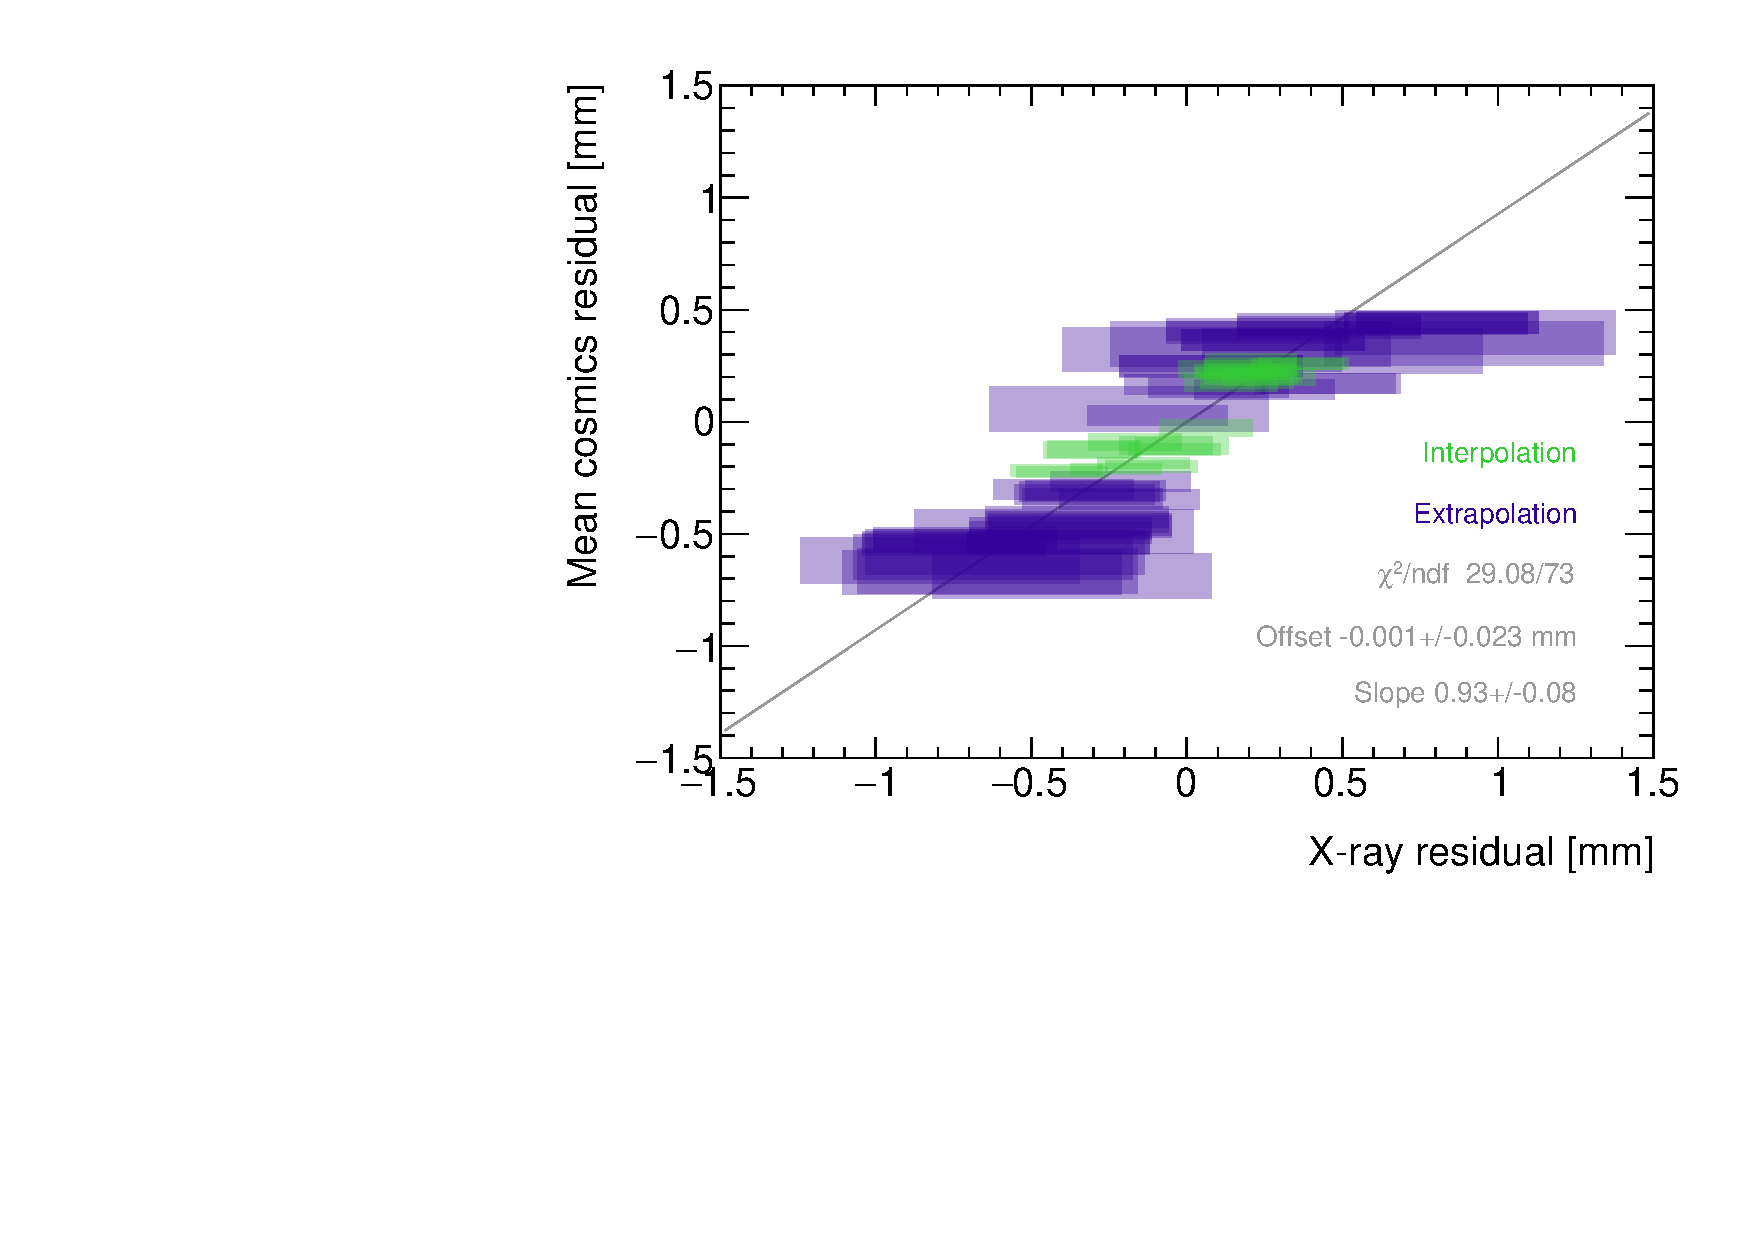
\includegraphics[width = \textwidth]{figures/figure_QL2P11_3100V_2021-08-05_QL2P11_local_cosmic_and_xray_data_correlation_plot.pdf}
    \caption{Correlation plot between x-ray and cosmics residuals for all tracking combinations for QL2.P.11. Each rectangle is centered on an x-ray and mean cosmics residual pair. The width of the rectangles in $x$ and $y$ are the uncertainty in the x-ray and mean cosmics residual respectively. A printer-friendly version of this plot is available in appendix~\ref{appendix:print}.}
    \label{fig:correlation}
\end{figure}

First, the fitted slope and offset in figure~\ref{fig:correlation} show that the two QL2.P.11 datasets are correlated. However, the magnitude of the uncertainties in the x-ray residuals is large (up to half a millimeter) since it comes from propagating the \SI{120}{\micro\meter} uncertainty in the beam profile centers. The large uncertainty set a limit on the sensitivity of the analysis, for if the absolute value of the x-ray residuals of a quadruplet were smaller than the x-ray residual uncertainties, no conclusion about the correlation could be drawn, like for QL2.P.8 (figure~\ref{fig:no_correlation}).

\begin{figure}
    \centering
    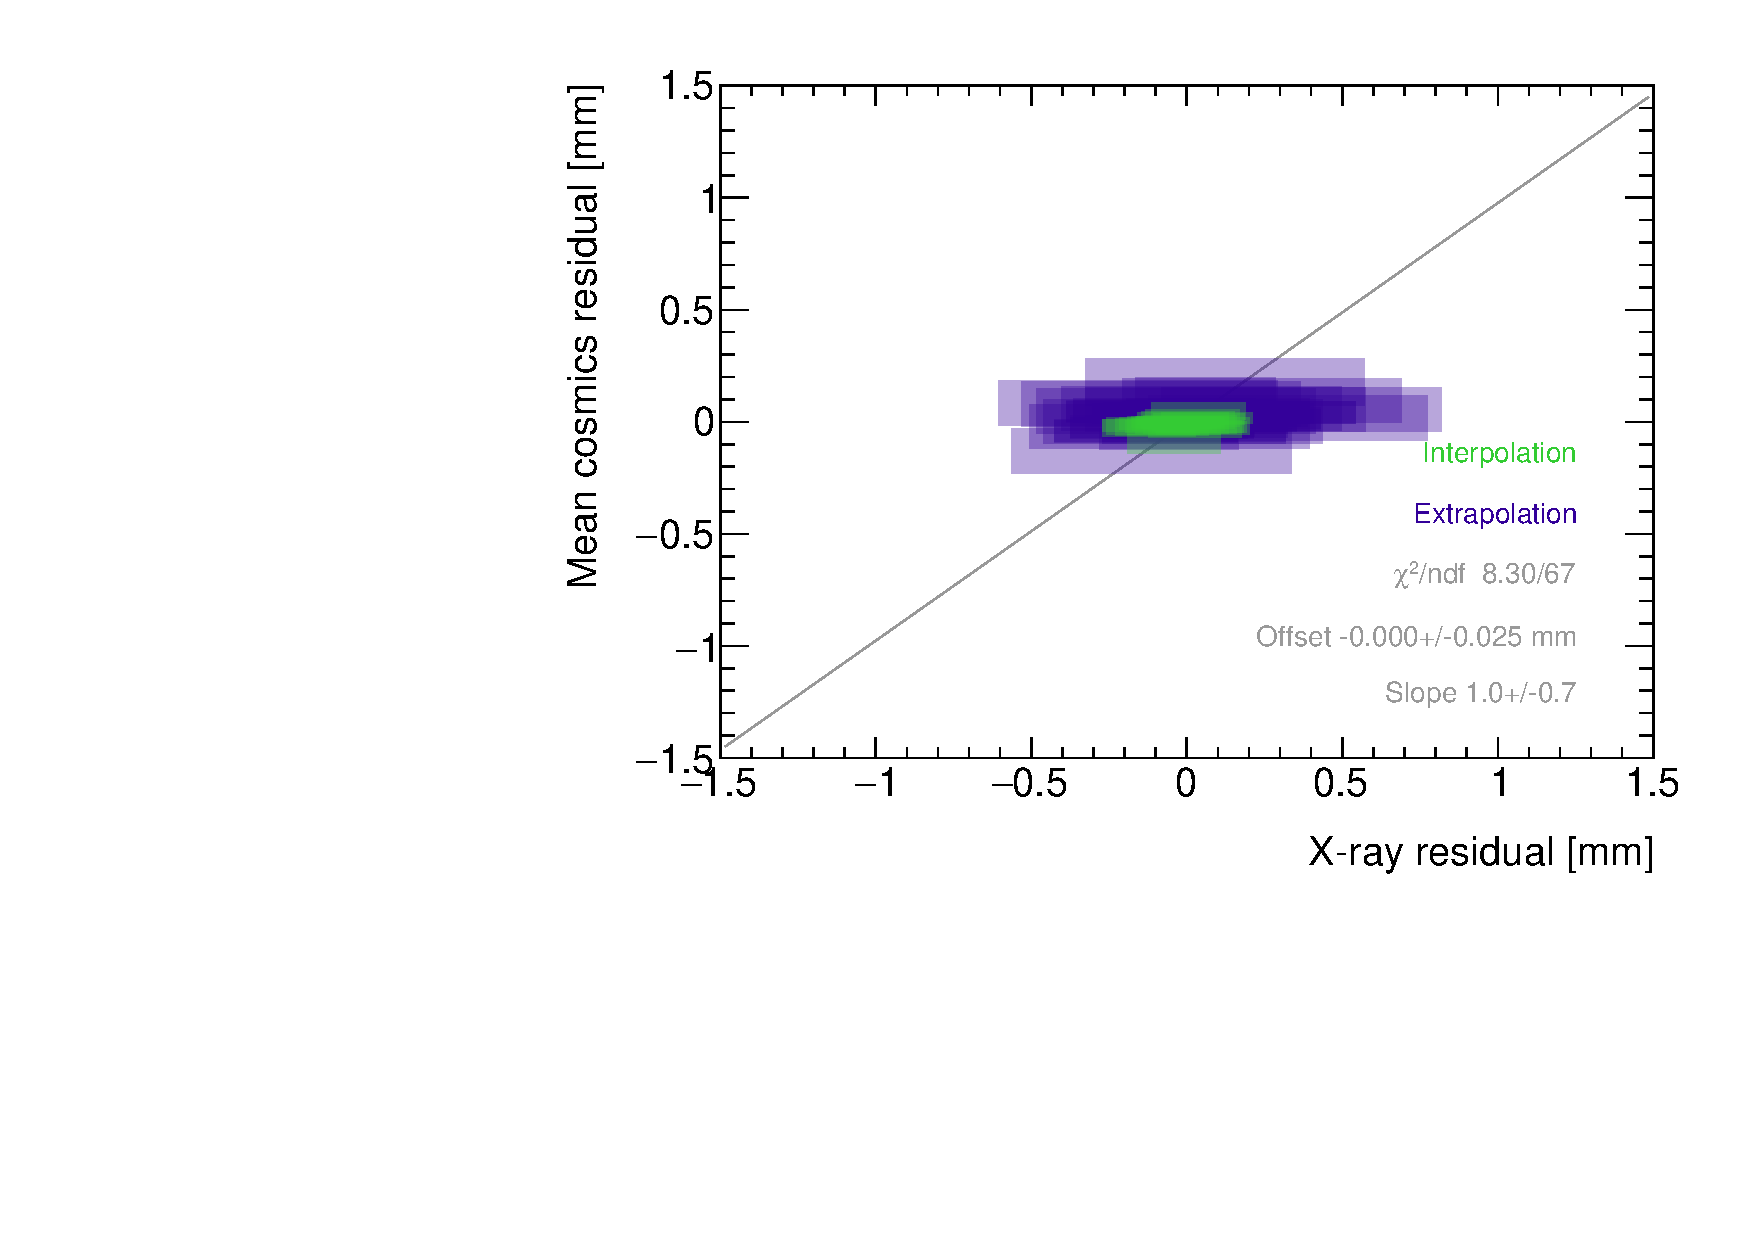
\includegraphics[width = \textwidth]{figures/figure_QL2P08_3100V_2021-08-16_QL2P08_local_cosmic_and_xray_data_correlation_plot.pdf}
    \caption{Correlation plot between x-ray and cosmics residuals for all tracking combinations for QL2.P.8. Each rectangle is centered on an x-ray and mean cosmics residual pair. The width of the rectangles in $x$ and $y$ are the uncertainty in the x-ray and mean cosmics residual respectively. A printer-friendly version of this plot is available in appendix~\ref{appendix:print}.}
    \label{fig:no_correlation}
\end{figure}

Several quadruplets were tested for each quadruplet construction geometry built in Canada: QL2P, QL2C, and QS3P. Each quadruplet fell into one of the two categories: residuals large enough to see a correlation, or residuals too small to see a correlation. Since the x-ray and mean cosmics residuals were measures of the relative local offsets between the layer of a quadruplet and the two reference layers, quadruplets with the most relative misalignment had the largest range of residuals. So, the correlation plots were an easy visual way to identify quadruplets with large relative misalignments.

There are three patterns in the residuals on the scatter plot explained by geometry. First, for both datasets the uncertainty in the extrapolated track residuals were larger than the interpolated track residuals because of the extrapolation lever arm. For the x-ray residuals, the effect of the lever arm on the uncertainty was direct since the residual was calculated from a single abstracted track; for the cosmics residuals it was the widening of the residual distribution on the layer of interest due to the extrapolation lever arm that increased the statistical uncertainty in the fitted mean of residuals. Second, residuals calculated through extrapolation tend to be larger because the extrapolation lever arm can produce more extreme values. Third, the pattern of points in figure~\ref{fig:correlation} is slightly mirrored. This is expected since the residuals calculated for a given set of three layers are geometrically correlated. 

The correlation of the cosmics residuals with the x-ray residuals alone does not validate the method; all the studies in described in appendices~\ref{appendix:statistics} and ~\ref{appendix:systematics} demonstrate its robustness. The analysis could be validated externally by comparing the mean cosmics residuals to the relative misalignment parameters calculated using \package{tgc\_analysis/MatrixMethod}~\cite{lefebvre_tgc_analysis} and JOHN FLORES CHI2 METHOD.

% --------------------------------------------------
\section{Limitations}
% --------------------------------------------------
The most important limit on measuring the degree of correlation between the x-ray and cosmics residuals was the uncertainty on the x-ray residuals, which stemmed from the systematic uncertainty in the x-ray beam profile centers~\cite{lefebvre_precision_2020}. The method was limited primarily by the sTGCs' poor x-ray position resolution, since x-rays do not create real tracks anyways. 

The analysis of certain quadruplets was also limited by the availability of data. Sometimes, less than three layers were surveyed for a given x-ray gun position so no residuals could be calculated. Too few x-ray residuals prevented the analysis from detecting a significant correlation. Often, the analysis of smaller quadruplets suffered as a result because they had fewer alignment platforms, and hence gun positions, on their surfaces. In addition, the analysis was limited to certain quadruplets. The wedges constructed the earliest (typically small wedges) were surveyed when the method was still being designed and so have limited x-ray residuals calculated from beam profiles of lower quality. Also, not all cosmic muon test sites had enough front end electronics to collect data on three layers simultaneously, which is the minimum required to be able to calculate residuals.

Nonetheless, the comparison of x-ray and cosmics residuals was really to confirm the x-ray local offsets with an independent dataset; the analysis of quadruplets with relative misalignments large enough to detect a correlation achieved this goal.


%----------------------------------------------------------------------
% END MATERIAL
% Bibliography, Appendices, Index, etc.
%----------------------------------------------------------------------

% Bibliography

% The following statement selects the style to use for references.  
% It controls the sort order of the entries in the bibliography and also the formatting for the in-text labels.
% Tony used unsrt in his PhD thesis
\bibliographystyle{unsrt}
% This specifies the location of the file containing the bibliographic information.  
% It assumes you're using BibTeX to manage your references (if not, why not?).
% \cleardoublepage % This is needed if the "book" document class is used, to place the anchor in the correct page, because the bibliography will start on its own page.
% Use \clearpage instead if the document class uses the "oneside" argument
\phantomsection  % With hyperref package, enables hyperlinking from the table of contents to bibliography             
% The following statement causes the title "References" to be used for the bibliography section:
\renewcommand*{\bibname}{References}

% Add the References to the Table of Contents
\addcontentsline{toc}{chapter}{\textbf{References}}

\bibliography{thesis}
% Tip: You can create multiple .bib files to organize your references. 
% Just list them all in the \bibliogaphy command, separated by commas (no spaces).

% The following statement causes the specified references to be added to the bibliography even if they were not cited in the text. 
% The asterisk is a wildcard that causes all entries in the bibliographic database to be included (optional).
\nocite{*}
%----------------------------------------------------------------------

% Appendices

% The \appendix statement indicates the beginning of the appendices.
\appendix
% Add an un-numbered title page before the appendices and a line in the Table of Contents
\chapter*{APPENDICES}
\addcontentsline{toc}{chapter}{APPENDICES}
% Appendices are just more chapters, with different labeling (letters instead of numbers).
%\chapter[TOC name for Acrobat Bookmarks sidebar]{Printed appendix title}
\chapter[PDF Plots From Matlab]{Matlab Code for Making a PDF Plot}
\label{appendix-example}
% Tip 4: Example (above) of how to get a shorter chapter title for the Table of Contents 
%======================================================================
\section{Using the Graphical User Interface}
Properties of Matab plots can be adjusted from the plot window via a graphical interface. Under the Desktop menu in the Figure window, select the Property Editor. You may also want to check the Plot Browser and Figure Palette for more tools. To adjust properties of the axes, look under the Edit menu and select Axes Properties.

To set the figure size and to save as PDF or other file formats, click the Export Setup button in the figure Property Editor.

\section{From the Command Line} 
All figure properties can also be manipulated from the command line. Here's an example: 
\begin{verbatim}
x=[0:0.1:pi];
hold on % Plot multiple traces on one figure
plot(x,sin(x))
plot(x,cos(x),'--r')
plot(x,tan(x),'.-g')
title('Some Trig Functions Over 0 to \pi') % Note LaTeX markup!
legend('{\it sin}(x)','{\it cos}(x)','{\it tan}(x)')
hold off
set(gca,'Ylim',[-3 3]) % Adjust Y limits of "current axes"
set(gcf,'Units','inches') % Set figure size units of "current figure"
set(gcf,'Position',[0,0,6,4]) % Set figure width (6 in.) and height (4 in.)
cd n:\thesis\plots % Select where to save
print -dpdf plot.pdf % Save as PDF
\end{verbatim}

% GLOSSARIES (Lists of definitions, abbreviations, symbols, etc. provided by the glossaries-extra package)
% -----------------------------
% \printglossaries
% \cleardoublepage
% \phantomsection		% allows hyperref to link to the correct page

%----------------------------------------------------------------------
\end{document} % end of logical document
